\chapter{Clusterização como um serviço} \label{cap:api}

  Uma solução para atender as necessidades do ``Empurrando Juntos'' é oferecer
  o processo de clusterização, juntamente com as funcionalidades de gerenciamento
  de conversas, comentários e votos, como um serviço.
  Uma forma de conseguir essa integração com o ``Empurrando Juntos'' é oferecer
  esses serviços através de uma \textit{Application Programming Interface} (API).

  De acordo com \citeonline{understanding_web}, uma API é uma interface que permite que os 
  usuários interajam ou respondam a dados ou serviços solicitados de outro programa, outros
  aplicativos ou sites. No contexto da Web, as APIs facilitam a troca de dados entre 
  aplicações, permitem a criação de novas aplicações e constituem a base para o conceito de 
  ``Web como uma plataforma''.

  \citeonline{wagh2012comparative} afirmam que existem vários métodos para interação entre o  
  usuário e a Internet, através de serviços web (web \textit{services}).
  Essa arquitetura permite que os componentes de software, o que inclui funções,
  objetos e processos de diferentes sistemas, sejam expostos como um serviço.

  Para prover esses serviços através de uma API, o estilo arquitetural Transferência de Estado 
  Representacional (do inglês, \textit{Representational State Transfer} ou REST)
  se destaca atualmente como representante do provimento de serviços via \textit{Web} e, portanto, foi escolhido para
  guiar a implementação da API proposta.

  O estilo REST é um estilo arquitetural introduzido por \citeonline{fielding2002} que serve como um modelo abstrato
  para guiar o uso do \textit{Hypertext Transfer Protocol} (HTTP) e do \textit{Uniform Resource Identifier} (URI)
  na arquitetura da Web moderna, abstraindo os elementos arquiteturais participantes de um sistema de
  hipermídia distribuído.
  
  \citeonline{perry1992} classificam os elementos arquiteturais em elementos de processamento (componentes),
  elementos de dados e elementos de conexão (conectores). O estilo REST foca no papel dos componentes, nas restrições
  da interação entre componentes e na interpretação de elementos de dados significantes para a interação \cite{fielding2002}.
  
  No estilo REST, uma informação é abstraída em um recurso, que pode ser qualquer informação que possa ser nomeada
  (documentos, imagens, serviços, entre outros). Para identificar um recurso específico na interação entre dois
  componentes, o REST utiliza um identificador de recurso (URI) \cite{fielding2002}.
  
  Componentes REST se comunicam transferindo uma representação do dado (informação) em algum formato padrão que pode
  ser selecionado dinamicamente com base nas preferências do destinatário \cite{fielding2002}. Além dos dados contidos na 
  informação, uma representação contém também metadados descrevendo os dados e, possivelmente, metadados sobre os
  metadados \cite{fielding2002}.
  
  \section{Maturidade de APIs RESTful}
  
      \citeonline{richardson09} propôs um modelo de maturidade para classificar
      APIs RESTful de acordo com os mecanismos da \textit{web} utilizados,
      que foi explicado de uma forma mais simples por \citeonline{fowler10}.
      A Figura \ref{fig:glory_of_rest}, apresentada por \citeonline{fowler10},
      ilustra os níveis do modelo de maturidade de \citeonline{richardson09}.
	
      \begin{figure}[h!]
	\centering
	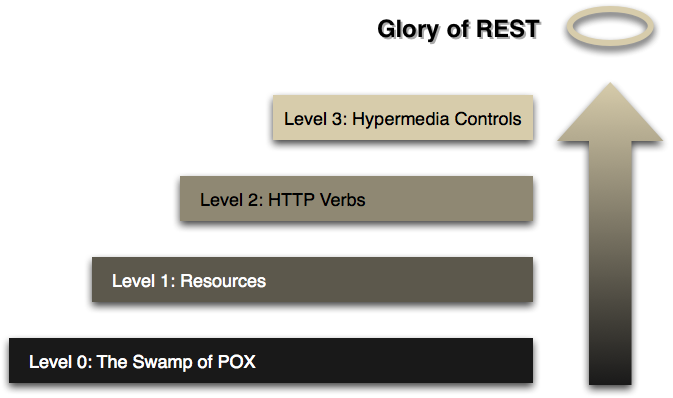
\includegraphics[scale=0.5]{figuras/glory_of_rest.png}
	\caption{Níveis do modelo de maturidade proposto por Richardson. Fonte: \cite{fowler10}}
	\label{fig:glory_of_rest}
      \end{figure}
      
      O nível zero consiste em utilizar o procotolo HTTP apenas como um meio de transporte de mensagens,
      comumente utilizando apenas um verbo HTTP e apenas um URI como ponto de entrada da API, 
      usando o HTTP com um túnel para uma comunicação remota \cite{fowler10} \cite{richardson09}.
      Essa característica é presenciada em APIs que implementam o protocolo \textit{Simple Object Access Protocol} (SOAP).
      
      O primeiro nível é alcançado quando se introduz o uso de recursos na API,
      o que permite identificar recursos individuais por meio URIs únicas,
      fornecendo pontos de entrada mais coesos para a API \cite{fowler10} \cite{richardson09}.
      
      O segundo nível é atingido quando a API utiliza da forma mais semântica possível
      os verbos e códigos de respostas providos pelo protocolo HTTP,
      fornecendo entradas e respostas mais semanticamente corretas \cite{fowler10} \cite{richardson09}.
      
      O terceiro e último nível é alcançado quando controles de hipermídia
      são introduzidos nas respostas da API \cite{fowler10} \cite{richardson09}.
      Este último nível, carinhosamente apelido de ``Glória do REST'' por \cite{fowler10},
      refere-se à restrição \textit{Hypertext As The Engine Of Application State} (HATEOAS) 
      que fornece meios (\textit{hyperlinks}) para informar ao cliente o que pode ser feito em seguida,
      para que ele possa navegar nos \textit{endpoints} da API de forma mais simples.
      
      Esta classificação permite identificar APIs boas e maduras para integração.
      